%!TEX root = ../main.tex

\chapter{Discussione}\label{chp:discussion}

Questo capitolo ha l'obiettivo di riassumere le caratterstiche principali dei tre tool discussi nel Capitolo\,\ref{chp:CNN-non-coding-variants} e compararne le prestazioni predittive 

I tre tool presentano alcune caratterstiche in comune. Si è scelto in tutti e tre i casi di utilizzare il \textsl{One Hot} encoding per codificare le sequenze in una matrice bidimensionale rendendo quindi immediata l'operazione di convoluzione in cui il kernel, per i tre tool è rappresentato da una \acs{PWM}. 

La struttura dei tre strumenti bioinformatici, anche se simile, presenta diverse differenze. 




cose identiche tra i tre tool:
- encode (one hot)
- loss function + training (lecito)

I tre tool bioinformatici hanno diverse caratterstiche in comune. La codifica scelta è la \textsl{One Hot encoding}, che divide . In secondo luogo 

\begin{itemize}
    \item 3 leayer convoluzionali, ciascuno dei quali seguito da una relu e da un max pooling
\end{itemize}


\begin{comment}
    \section{Codifica}
    
    \section{Struttura della rete}
    
    \section{Dataset}
\end{comment}


\begin{table}[!h]
    \centering
    \renewcommand{\arraystretch}{2}
    \begin{tabular}{|c|c|c|c|c|c|} % chktex-file 44
        \hline % chktex-file 44
        \textbf{Modello} & \textbf{Struttura} & \textbf{Codifica} & \textbf{Numero kernel} & \textbf{Dataset} \\ 
        \hline\hline % chktex-file 44
        \hyperref[sec:DeepSEA]{\textsl{DeepSEA}} & & One-hot Encoding & \acs{PWM} & Lesgoschi \\ 
        % 
        \hyperref[sec:Basset]{\textsl{Basset}} & & One-hot Encoding & \acs{PWM} & Lesgoschi \\ 
        % 
        \hyperref[sec:DeepSATA]{\textsl{DeepSATA}} & & One-hot Encoding & \acs{PWM} & Lesgoschi \\ 
        \hline
    \end{tabular}
    \renewcommand{\arraystretch}{1}
\end{table}


\todo{Fai un paragrafo struttura}
\todo{Tabella che contiene: input richiesto ($1000 \times 4$,  $600 \times 4$ e  $1000 \times 4 \times 10 + 1$), dataset scelto}

Questi qua sono i risultati, guarda DeepSATA

\begin{table}[!h]
    \centering
    \renewcommand{\arraystretch}{2}
    \begin{tabular}{|c|c|c|c|c|c|} % chktex-file 44
        \hline % chktex-file 44
        \textbf{Modello} & \textbf{Topi} & \textbf{Maiali} & \textbf{Bovini} & \textbf{Umani} & \textbf{Polli}\\ 
        \hline\hline % chktex-file 44
        \hyperref[sec:DeepSEA]{\textsl{DeepSEA}} & 0.796 & 0.775 & 0.769 & 0.755 & 0.736 \\ 
        % 
        \hyperref[sec:Basset]{\textsl{Basset}} & 0.778 & 0.719 & 0.768 & 0.717 & 0.722 \\ 
        % 
        \hyperref[sec:DeepSATA]{\textsl{DeepSATA}} & 0.854 & 0.779 & 0.772 & 0.759 & 0.744 \\ 
        \hline
    \end{tabular}
    \renewcommand{\arraystretch}{1}
\end{table}


\begin{figure}[!b]
    \centering
    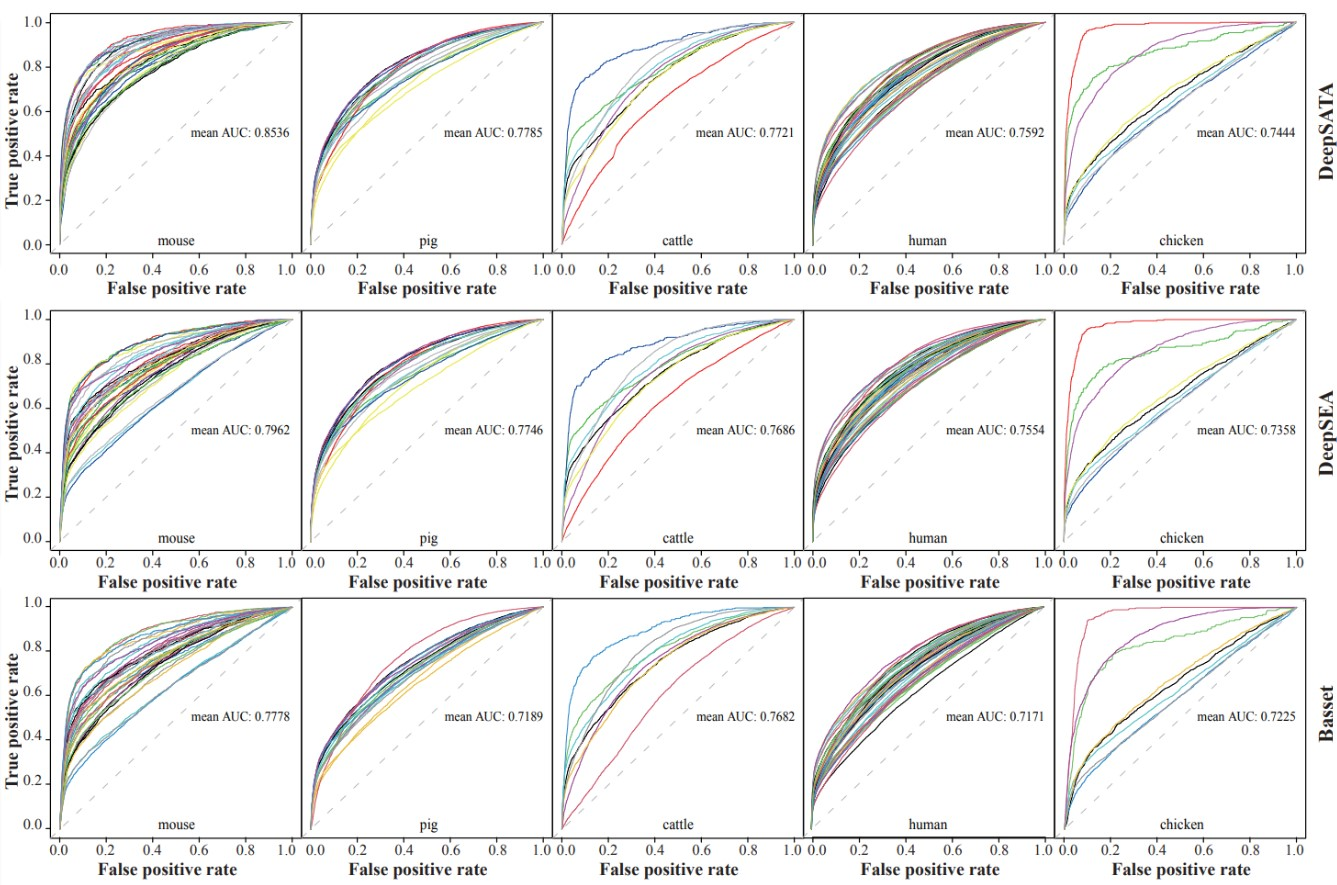
\includegraphics[width=1\textwidth]{assets/imgs/comparison.jpg}
    \caption[Confronto delle prestazioni predittive dei tre tool su diverse specie animali.]{Confronto delle prestazioni predittive dei tre tool su diverse specie animali.}\label{fig:comparison}
\end{figure}

\todo{Tabella che specifica e riassume per ogni tool encoding, dataset etc}
\todo{riassume quanto analizzato prima, riporta i risultati del paper piu recente in modo da avere un momento in cui riassumo la situa}
\todo{Sperimentalmente, per risorse a disposizione, per il confronto ci si basa sui risultati dell'ultimo paper}

\begin{comment}
    In our study, we utilized DeepSATA to evaluate its predictive capabilities for chromatin features in five distinct species: mice, pigs, cattle, humans, and chickens. We collected open chromatin accessibility datasets and corresponding transcription factor binding motifs, which are summarized in Table 1 and Supplementary Tables S1 and S2. The performance of the DeepSATA, DeepSEA, and Basset models was assessed for each species by comparing their average AUC values across different chromatin features. DeepSATA demonstrated superior performance across all species, with average AUC values of 0.854, 0.779, 0.772, 0.759, and 0.744 for mice, pigs, cattle, humans, and chickens, respectively (Figure 2A and Supplementary Table S3). In comparison, DeepSEA had average AUC values of 0.796, 0.775, 0.769, 0.755, and 0.736, respectively (Figure 2B and Supplementary Table S3), while Basset had average AUC values of 0.778, 0.719, 0.768, 0.717, and 0.722, respectively (Figure 2C and Supplementary Table S3). It is worth noting that DeepSATA consistently outperformed DeepSEA and Basset in all chromatin features for pigs and mice (Supplementary Table S3). The relative improvement was particularly significant in the cerebrum tissue of the mice, where DeepSATA achieved an AUC of 0.829 compared to DeepSEA’s 0.659 for female mice and an AUC of 0.828 compared to DeepSEA’s 0.653 for male mice, representing a relative improvement of over 25%. Interestingly, our findings indicate that the DeepSATA, DeepSEA, and Basset models performed better for the Duroc pig breed compared to other pig breeds (Supplementary Table S3). This suggests a superior ability to recognize regulatory functional patterns in the non-coding genomic regions  pecific to Duroc pigs. In the case of cattle, the chromatin feature of the hypothalamus was most effectively captured, with AUC values of 0.887 for DeepSATA, 0.883 for DeepSEA, and 0.895 for Basset (Supplementary Table S3). What particularly encouraged us was the remarkable performance of DeepSATA in accurately recognizing the regulatory patterns of the cerebellum in chickens, achieving AUC values as high as 0.972, while DeepSEA achieved 0.971 and Basset achieved 0.953 (Supplementary Table S3). Additionally, in the following analysis, we selected DeepSEA as the baseline comparison, since it achieved better prediction performance compared with Basset. Overall, these results clearly demonstrate the effectiveness of DeepSATA in accurately identifying the regulatory patterns of chromatin features in different animal species
\end{comment}
